\section{gyakorlat (2025. október 15.)}
\subsubsection*{Még egy geometriai oszd meg és uralkodj algoritmus (igazából összefésülés variáció)}
\begin{figure}[H]
  \includegraphics[width=5cm]{gy/img/gy06_skyline1}
\end{figure}
$n$ téglalap, amelyek az $x$ tengelyen állnak

Feladat: sziluett (felső burkoló töröttvonal) meghatározása.

Téglalapok: $T_1, T_2, \cdots, T_n$

\begin{tikzpicture}
\draw[->] (-0.5, 0) -- (4, 0);
\draw[->] (0, -0.5) -- (0, 3);

\draw[dashed] (0, 2) -- (1, 2);
\draw (1, 2) -- (2, 2);
\draw (1, 0) -- (1, 2); 
\draw (2, 0) -- (2, 2);

\node at (-0.3, 2){$y_i$};
\node at (1, -0.3){$x'_i$};
\node at (2, -0.3){$x''_i$};
\node at (1.5, 1){$T_i$};
\node at (4, 1){$T_i \leftrightarrow (x'_i, y_i, x''_i)$};
\end{tikzpicture}

Sziluett

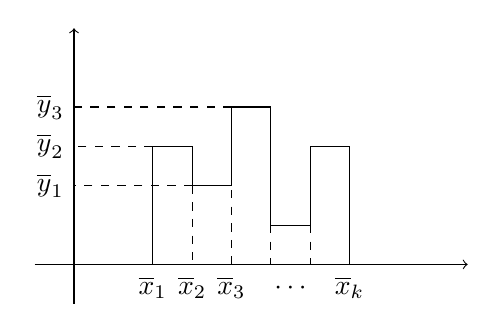
\begin{tikzpicture}
\draw[->] (-0.5, 0) -- (5, 0);
\draw[->] (0, -0.5) -- (0, 3);

\draw (1, 0) -- (1, 1.5);
\draw (1, 1.5) -- (1.5, 1.5);
\draw (1.5, 1.5) -- (1.5, 1);
\draw (1.5, 1) -- (2, 1);
\draw (2, 1) -- (2, 2);
\draw (2, 2) -- (2.5, 2);
\draw (2.5, 2) -- (2.5, 0.5);
\draw (2.5, 0.5) -- (3, 0.5);
\draw (3, 0.5) -- (3, 1.5);
\draw (3, 1.5) -- (3.5, 1.5);
\draw (3.5, 1.5) -- (3.5, 0);

\draw[dashed] (2, 2) -- (0, 2);
\draw[dashed] (2, 2) -- (2, 0);
\draw[dashed] (1, 1.5) -- (0, 1.5);
\draw[dashed] (1, 1.5) -- (1, 0);
\draw[dashed] (1.5, 1) -- (0, 1);
\draw[dashed] (1.5, 1) -- (1.5, 0);
\draw[dashed] (2.5, 0.5) -- (2.5, 0);
\draw[dashed] (3, 0.5) -- (3, 0);

\node at (-0.3, 2){$\overline{y}_3$};
\node at (-0.3, 1.5){$\overline{y}_2$};
\node at (-0.3, 1){$\overline{y}_1$};

\node at (1, -0.3){$\overline{x}_1$};
\node at (1.5, -0.3){$\overline{x}_2$};
\node at (2, -0.3){$\overline{x}_3$};
\node at (2.75, -0.3){$\cdots$};
\node at (3.5, -0.3){$\overline{x}_k$};
\end{tikzpicture}

$(\overline{x}_1, \overline{y}_1, \overline{x}_2, \overline{y}_2, \cdots, \overline{y}_{k-1}, \overline{x}_k)$

\textbf{Oszd meg és uralkodj algoritmus}\\
\begin{enumerate}
    \item Két feleakkora méretű részfeladat
    \begin{itemize}
    \item $T_1 ,T_2, \cdots, T_{n/2}$ sziluettjének meghatározása
    \item $T_{n/2 + 1} ,T_{n/2 + 2}, \cdots, T_{n}$ sziluettjének meghatározása
    \end{itemize}
    \item Rekurzívan megoldjuk a részfeladatokat (egy téglalap esetén triviális)
    \item Összekombináljuk a két sziluettet:
    \begin{figure}[H]
        \includegraphics[width=5cm]{gy/img/gy06_skyline2}
    \end{figure}
    (ez már egy összefésülés)
\end{enumerate}
Minden szakaszon a magasabban fekvő szakaszt választjuk a két sziluetten.


Implementáljuk ezt ha tényleg minden részletében érteni szeretnénk.

Költség: $T(n) = 2T(\frac{n}{2}) + \mathcal{O}(n) \rightarrow T(n) = \mathcal(O)(n \log n)$


\subsection{Érmék egy sorban (tegnapi előadás)}
(Ez már nem oszd meg és uralkodj)

\begin{tikzpicture}[
    roundnode/.style={circle, draw=black, minimum size=0.7cm, inner sep=0.5mm}
]
\node[roundnode](c1){$c_1$};
\node[roundnode](c2)[right = 0.2cm of c1]{$c_2$};
\node[roundnode](c3)[right = 0.2cm of c2]{$c_3$};
\node[roundnode](c4)[right = 0.2cm of c3]{$c_4$};
\node(cdots)[right = 0.2cm of c4]{$\cdots$};
\node[roundnode](c2n1)[right = 0.2cm of cdots]{$c_{2n-1}$};
\node[roundnode](c2n)[right = 0.2cm of c2n1]{$c_{2n}$};   
\end{tikzpicture}

Egy sorban $2n$ (nem feltétlenül páronként) különböző érmék vannak.
Két játékos felváltva elvesz a (megmaradt) érmék sorának valamelyik végéről egy érmét.
Az győz, akinél az elvett érmék értékének összege nagyobb.

Először is: döntetlen lehetséges.
\begin{tikzpicture}[
    roundnode/.style={circle, draw=black, minimum size=0.6cm, inner sep=0.5mm}
]
\node[roundnode](c1){$1$};
\node[roundnode](c2)[right = 0.2cm of c1]{$1$};
\node[roundnode](c3)[right = 0.2cm of c2]{$1$};
\node[roundnode](c4)[right = 0.2cm of c3]{$1$};
\node[roundnode](c5)[right = 0.2cm of c4]{$1$};
\node[roundnode](c6)[right = 0.2cm of c5]{$1$};
\end{tikzpicture}

A nyerő stratégia a nem vesztő stratégia.

Nyerő stratégia a kezdő számára: tud úgy érmét elvenni először, hogy erre "bármit lép" a másik játékos, a kezdő megint tud úgy érmét elvenni, hogy erre "bármit lép" a másik játékos, \cdots, a kezdő nyer (nem veszít)

Nyerő stratégia a másik játékosnak: bármit lép a kezdő játékos, a másik játékos tud úgy érmét elvenni, hogy erre bármit lép a kezdő játékos, a másik tud úgy érmét elvenni, \cdots, a másik játékos nyer (nem veszít).

Ebben a játékban a kezdőnek van nyerő (nem vesztő) stratégiája!

\setstcolor{black}
\begin{tikzpicture}[
    roundnode/.style={circle, draw=black, minimum size=0.6cm, inner sep=0.5mm}
]
\node[roundnode](c1){$7$};
\node[roundnode](c2)[right = 0.2cm of c1]{$8$};
\node[roundnode](c3)[right = 0.2cm of c2]{$6$};
\node[roundnode](c4)[right = 0.2cm of c3]{$7$};
\node[roundnode](c5)[right = 0.2cm of c4]{$9$};
\node[roundnode](c6)[right = 0.2cm of c5]{$8$};
\node[roundnode](c7)[right = 0.2cm of c6]{$6$};
\node[roundnode](c8)[right = 0.2cm of c7]{$7$};

\draw (-0.3, -0.3) -- ++(0.6, 0.6);
\draw (-0.3, 0.3) -- ++(0.6, -0.6);

\draw (0.5, -0.3) -- ++(0.6, 0.6);
\draw (0.5, 0.3) -- ++(0.6, -0.6);

\draw (1.3, -0.3) -- ++(0.6, 0.6);
\draw (1.3, 0.3) -- ++(0.6, -0.6);

\draw (2.15, -0.3) -- ++(0.6, 0.6);
\draw (2.15, 0.3) -- ++(0.6, -0.6);

\draw (2.95, -0.3) -- ++(0.6, 0.6);
\draw (2.95, 0.3) -- ++(0.6, -0.6);

\draw (3.75, -0.3) -- ++(0.6, 0.6);
\draw (3.75, 0.3) -- ++(0.6, -0.6);

\draw (4.6, -0.3) -- ++(0.6, 0.6);
\draw (4.6, 0.3) -- ++(0.6, -0.6);

\draw (5.4, -0.3) -- ++(0.6, 0.6);
\draw (5.4, 0.3) -- ++(0.6, -0.6);
\end{tikzpicture}

Kezdő (összesen 30):
\begin{tikzpicture}[
    roundnode/.style={circle, draw=black, minimum size=0.6cm, inner sep=0.5mm}
]
\node[roundnode](c1){$7$};
\node[roundnode](c2)[right = 0.2cm of c1]{$8$};
\node[roundnode](c3)[right = 0.2cm of c2]{$6$};
\node[roundnode](c4)[right = 0.2cm of c3]{$9$};
\end{tikzpicture}

Másik (összesen 28):
\begin{tikzpicture}[
    roundnode/.style={circle, draw=black, minimum size=0.6cm, inner sep=0.5mm}
]
\node[roundnode](c1){$7$};
\node[roundnode](c2)[right = 0.2cm of c1]{$6$};
\node[roundnode](c3)[right = 0.2cm of c2]{$8$};
\node[roundnode](c4)[right = 0.2cm of c3]{$7$};
\end{tikzpicture}

A kezdő játékos ki tudja kényszeríteni, hogy a másik csak a páros indexű $c_i$-ket és azt is hogy csak a páratlan indexű $c_i$-ket vegye el (az összeset).

Pl. a páros indexekre:

\begin{tikzpicture}[
    roundnode/.style={circle, draw=black, minimum size=0.6cm, inner sep=0.5mm}
]
\node[roundnode](c1_1) at (0, 0) {$c_1$};

\node[roundnode](c2_1) at (2, 2) {$c_2$};
\node[roundnode](c2_2) at (2, -2) {$c_8$};

\node[roundnode](c3_1) at (4, 2) {$c_3$};
\node[roundnode](c3_2) at (4, -2) {$c_7$};

\node[roundnode](c4_1) at (6, 3) {$c_4$};
\node[roundnode](c4_2) at (6, 1) {$c_8$};
\node[roundnode](c4_3) at (6, -1) {$c_2$};
\node[roundnode](c4_4) at (6, -3) {$c_6$};

\node[roundnode](c5_1) at (8, 3) {$c_5$};
\node[roundnode](c5_2) at (8, 1) {$c_7$};
\node[roundnode](c5_3) at (8, -1) {$c_3$};
\node[roundnode](c5_4) at (8, -3) {$c_5$};

\node[roundnode](c6_1) at (10, 3.5) {$c_6$};
\node[roundnode](c6_2) at (10, 2.5) {$c_8$};
\node[roundnode](c6_3) at (10, 1.5) {$c_4$};
\node[roundnode](c6_4) at (10, 0.5) {$c_6$};
\node[roundnode](c6_5) at (10, -0.5) {$c_4$};
\node[roundnode](c6_6) at (10, -1.5) {$c_6$};
\node[roundnode](c6_7) at (10, -2.5) {$c_2$};
\node[roundnode](c6_8) at (10, -3.5) {$c_4$};

\node[roundnode](c7_1) at (12, 3.5) {$c_7$};
\node[roundnode](c7_2) at (12, 2.5) {$c_7$};
\node[roundnode](c7_3) at (12, 1.5) {$c_5$};
\node[roundnode](c7_4) at (12, 0.5) {$c_5$};
\node[roundnode](c7_5) at (12, -0.5) {$c_5$};
\node[roundnode](c7_6) at (12, -1.5) {$c_5$};
\node[roundnode](c7_7) at (12, -2.5) {$c_3$};
\node[roundnode](c7_8) at (12, -3.5) {$c_3$};

\draw[-Stealth] (c1_1) -- (c2_1);
\draw[-Stealth] (c1_1) -- (c2_2);

\draw[-Stealth] (c2_1) -- (c3_1);
\draw[-Stealth] (c2_2) -- (c3_2);

\draw[-Stealth] (c3_1) -- (c4_1);
\draw[-Stealth] (c3_1) -- (c4_2);
\draw[-Stealth] (c3_2) -- (c4_3);
\draw[-Stealth] (c3_2) -- (c4_4);

\draw[-Stealth] (c4_1) -- (c5_1);
\draw[-Stealth] (c4_2) -- (c5_2);
\draw[-Stealth] (c4_3) -- (c5_3);
\draw[-Stealth] (c4_4) -- (c5_4);

\draw[-Stealth] (c5_1) -- (c6_1);
\draw[-Stealth] (c5_1) -- (c6_2);
\draw[-Stealth] (c5_2) -- (c6_3);
\draw[-Stealth] (c5_2) -- (c6_4);
\draw[-Stealth] (c5_3) -- (c6_5);
\draw[-Stealth] (c5_3) -- (c6_6);
\draw[-Stealth] (c5_4) -- (c6_7);
\draw[-Stealth] (c5_4) -- (c6_8);

\draw[-Stealth] (c6_1) -- (c7_1);
\draw[-Stealth] (c6_2) -- (c7_2);
\draw[-Stealth] (c6_3) -- (c7_3);
\draw[-Stealth] (c6_4) -- (c7_4);
\draw[-Stealth] (c6_5) -- (c7_5);
\draw[-Stealth] (c6_6) -- (c7_6);
\draw[-Stealth] (c6_7) -- (c7_7);
\draw[-Stealth] (c6_8) -- (c7_8);

\node[below=0.5cm of c1_1]{kezdő};
\node[below=0.5cm of c3_2]{kezdő};
\node[below=0.5cm of c5_4]{kezdő};
\node[below=0.5cm of c7_8]{kezdő};
\end{tikzpicture}


Ezek után a nyerő stratégia:\\
$S_{ps} := c_2 + c_4 + c_6 + \cdots + c_{2n}$\\
$S_{plan} := c_1 + c_3 + c_5 + \cdots + c_{2n-1}$

Ha $S_{ps} \leq S_{plan}$, akkor a kezdő mindig a páratlan indexű érméket vegye el, különben mindig a páros indexűeket.

Példánkban:\\
$S_{ps} = 8 + 7 + 8 + 7 = 30$\\
$S_{plan} = 7 + 6 + 9 + 6 = 28$\\
A kezdőnek a páros indexű érméket kell elvenni.

Optimális ez?
Nem feltétlenül.\\
Új kérdés: milyen stratégiát kövessen a kezdő, hogy a különbség a javára maximális legyen?
Az előző példánál a második játékosnak (globálisan) nem volt mozgástere.
Általában ez nincs így.

Optimális stratégia a kezdő számára: bárhogy játszik a másik, a különbség mindenképp meglesz.
Aprópénzre váltva: a másik "optimális stratégiája" mellett is (a másik játékos optimális stratégiája: minimalizálni akarja a különbséget).



